\documentclass[a4paper]{article}

\setcounter{tocdepth}{1}

\usepackage{color}
\usepackage{url}
\usepackage[T2A]{fontenc} % enable Cyrillic fonts
\usepackage[utf8]{inputenc} % make weird characters work
\usepackage{graphicx}
\usepackage{subcaption}
\usepackage{amsmath}

\usepackage[english,serbianc]{babel}

\usepackage[unicode]{hyperref}
\hypersetup{colorlinks,citecolor=green,filecolor=green,linkcolor=blue,urlcolor=blue}

\usepackage{listings}

\definecolor{mygreen}{rgb}{0,0.6,0}
\definecolor{mygray}{rgb}{0.5,0.5,0.5}
\definecolor{mymauve}{rgb}{0.58,0,0.82}

\lstset{ 
  backgroundcolor=\color{white},
  basicstyle=\scriptsize\ttfamily,  
  breakatwhitespace=false,         
  breaklines=true,                 
  captionpos=b,                   
  commentstyle=\color{mygreen},   
  deletekeywords={...},           
  escapeinside={\%*}{*)},          
  extendedchars=true,              
  firstnumber=1000,                
  frame=single,	                   
  keepspaces=true,                 
  keywordstyle=\color{blue},       
  language=Python,                 
  morekeywords={*,...},            
  numbers=left,                    
  numbersep=5pt,                   
  numberstyle=\tiny\color{mygray},
  rulecolor=\color{black},        
  showspaces=false,               
  showstringspaces=false,          
  showtabs=false,                  
  stepnumber=2,                   
  stringstyle=\color{mymauve},     
  tabsize=2,	                   
  title=\lstname                   
}

\begin{document}

\title{\Large Рибарење\\ \small{Научни рад у оквиру курса Основе математичког моделирања\\ Универзитет у Београду, Математички факултет}}

\author{Душан Пантелић\\ pantelic.dusan@protonmail.com}

\maketitle

\begin{center}
	
\includegraphics[width=3cm]{images/pmf.png}
\end{center}

\abstract{
Кроз овај рад читалац ће бити упућен у проблем рибарења, као и у математичко моделовање и решавање истог. Пре свега, шта представља проблем рибарења, његов значај, примену, али и проблеме при проналажењу оптимума и стања равнотеже модела. Представљене су формуле за одрећивања стања еквилибријума. Читалац ће такође добити увид у експерименталне податке на основу приказаног модела и решења приказаних у раду. На крају рада сумирани су закључци истраживања и изложени правци за даље истраживање и унапређивање.
\tableofcontents

\newpage

\section{Увод}
\label{sec:intro}
Математичким моделирањем рибарења за циљ имамо одређивање оптималног броја уловљене рибе у неком станишту тако да успоставимо равнотежу и не угрозимо опстанак рибе у том станишту, али и задовољимо потребе рибара. Решење горе наведеног проблема се користи и за одређивање квота тј. максималног дозвољеног броја уловљене рибе на неком подручју. Претпоставићемо да ограничен број ресусрса у станишту рибе утиче на величину популације рибе, као и број људи који се бави рибарењем. Величина популације рибе ће такође утицати на број рибара јер при недостатку рибе део рибара ће престати да се бави тим послом због економске неисплативости, али и приликом веће количине рибе биће већи број људи који ће почети да се баве тим послом. Нећемо узимати у обзир комплексније факторе као што су други предатори који такође лове рибу, економске факторе попут презасићења тржишта, понуде и потражње и друге.

\section{Популација рибе без рибарења}
\label{sec:nofishing}
За моделирање рибље популације без присуства рибара користићемо Верхулстов логистички модел.
\begin{equation}
    \frac{dN(t)}{dt} = rN(t)\left(1-\frac{N(t)}{K}\right)
\end{equation}
Из горе наведеног модела видимо да број рибе у неком трентку $N(t)$ зависи од стопе раста $r$, као и од оптималног броја рибе у станишту $K $ тако да има довољно ресурса за све. Решавањем овог модела добијамо следећу једначину:
\begin{equation}
    N(t) = \frac{N(0)e^r^t}{1+\frac{N(0)}{K}(e^r^t - 1)}
\end{equation}
Како би смо симулирали популацију рибе кроз време претпоставићемо да се риба налази у рибњаку и да су нам финансије ограничавајући фактор тако да максимално можемо купити хране за $10000$ риба што нам представља горе наведену константу $K$. Природни прираштај рибе од 30\% представићемо константом $r=0.3$, такође ћемо претпоставити да је постојало почетно улагање од 1000 риба што је почетна популација у рибњаку тј. $N(0)$. Симулацију броја рибе у наредних 50 година можемо видети на слици \ref{fishnofishing_view}.
\begin{figure}[h!]
	\centering
	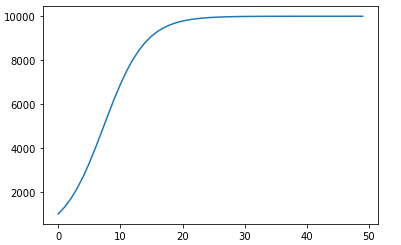
\includegraphics[width=10cm,height=3.5cm]{images/FishPopulationNoFishing.png}
	\caption{Популација рибе без рибарења}
	\label{fishnofishing_view}
\end{figure}
Mожемо приметити да након неког времена популација рибе тежи константи $K$, као и да прираштај нема ефекта због ограничења ресурса.

\section{Математички модел рибарења}
\label{sec:fishing}
Како би смо имали увид о популацији рибе али и рибара, промене њихових популација и њихову међусобну интеракцију моделираћемо допуњеним Лотка-Волтеровим моделом (\ref{modifiedLV1} и \ref{modifiedLV2} ) за грабљивце и плен.
\begin{equation}
    \label{modifiedLV1}
    \frac{dP(t)}{dt} = rP(t)\left(1-\frac{P(t)}{K}\right) - gP(t)G(t)
\end{equation}
\begin{equation}
    \label{modifiedLV2}
    \frac{dG(t)}{dt} = lgP(t)G(t) - hG(t)
\end{equation}

У првом делу модела (\ref{modifiedLV1}) представљена је популација плена тј. рибе током времена, док је у другом делу (\ref{modifiedLV2}) представљена популација рибара.
\begin{itemize}
  \item $ rP(t)\left(1-\frac{P(t)}{K}\right)$ представља логистички модел дефинисан у претходном делу
  \item $gP(t)G(t)$ је количина уловљене рибе зависне од константе $g$ која представља интензитет риболова, као и производа популације рибе и рибара који представља њихову међусобну интеракцију.
  \item $lgP(t)G(t)$ представља нове рибаре који су због доста улова кренули да се баве том професијом. Константа $l$ преставља фактор који на основу броја уловљене рибе одређује број нових рибара.
  \item $hG(t)$ представља број рибара који престају да се баве рибарењем због недостатка рибе.
  
\end{itemize}
Нумеричко решење модела за параметре $[P(0)=1000, G(0)=100, K=1000, r=0.5, g=0.001, l=0.5, h=0.75] $ можемо видети слици \ref{sec:fishing} која нам приказује промену величине популације рибе и рибара у периоду од 50 година. Можемо приметита да популације осцилују међусобно пропорционалним интензитетом периодично, са тим да је приметан померај осцилације популације рибара у односу на популације рибе. Такође за разлику од класичног Лотка-Волтеровог модела имамо мање интензите осцилација због коришћења логистичке функције за популацију рибе уместо експоненциалне. У претходном поглављу \ref{sec:nofishing} смо видели да на графику \ref{sec:nofishing} када нема рибарења популација рибе достиже свој максимум, док на графику модела рибарења видимо да иако је параметар раста популације рибе $r$ већи популација рибе не достиже свој максимум због већег интензитета риболова.

 \begin{figure}[h!]
	\centering
	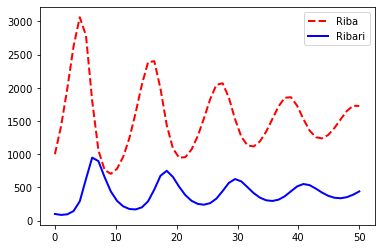
\includegraphics[width=10cm,height=4.5cm]{images/FishPopulationFishing.png}
	\caption{Популација рибе и рибара}
	\label{fishfishing_view}
\end{figure}

\section{Оптимална количина уловљене рибе}
\label{sec:fishingoptimum}
Како би наш претходно дефинисани модел у пракси био одржив на дужи временски период потребно је успоставити равнотежу између броја рибе и рибара у зависности од вредности параметара модела. Не желимо прекомерну количину рибе која ће умирати због недостатака ресурса, али такође не желимо ни превелики број рибара који ће можда истребити рибу. Такође још један од битних параметара је интензитет риболова који мора бити оптимално одабран.

За проналазак оптималног случаја користиће нам стања равнотеже модела тј. еквилибријуми. Еквилибријуме добијамо решавањем система једначина приказаним у (\ref{eqpt1} и \ref{eqpt2}).
\begin{equation}
    \label{eqpt1}
    rP\left(1-\frac{P}{K}\right) - gPG  = 0
\end{equation}

\begin{equation}
    \label{eqpt2}
    lgPG - hG = 0
\end{equation}
Решавањем система добијамо три еквилибријума $E(0,0), E(K,
0)$ и $E(\frac{h}{gl},\frac{(gKl - h)*r}{g^2Kl})$. Прва два еквилибријума су редом случајеви када не постоје ни риба ни рибари, и риба са почетном популацијом К без рибара тако да та два еквилибријума нећемо даље разматрати већ ћемо се фокусирати на последњи еквилибријум. 

\begin{figure}[h!]
	\centering
	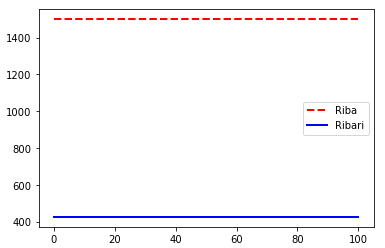
\includegraphics[width=10cm,height=4.6cm]{images/equilibrium1.png}
	\caption{Почетни еквилибријум}
	\label{equilibrium1}
\end{figure}

\begin{figure}[h!]
	\centering
	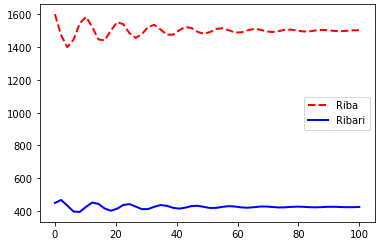
\includegraphics[width=10cm,height=4.6cm]{images/equilibrium2.png}
	\caption{Успостављени еквилибријум}
	\label{equilibrium2}
\end{figure}

На слици \ref{equilibrium1} видимо график популације рибе и рибара кад за почетне популације поставимо вредности тачке еквилибријума. Такође на слици \ref{equilibrium2} видимо да ће при вредностима блиским еквилибријуму популације после неког времена постићи равнотежус.

Иако претходно описаним поступком постижемо равнотежу система, реалнија је ситуација у којој знамо приближан број рибе у рибњаку, а на основу тога одређујемо дозвољени број рибара и оптималан интензитет риболова тако да систем без већих осцилација постиже равнотежу. 
За решење претходно описаног проблема користићемо систем једначина (\ref{eqpt1} и \ref{eqpt2}), са тим што ћемо сада уз $P$ i $G$ сматрати да је непознато и $h(P,G)$ што нам представља број уловљене рибе тј. $gPG$ . За овако дефинисан систем добијамо тачку еквилибријума $E(P = P0, G = \frac{P0Kr-P0^2r}{K}, h(P,G) = \frac{P0Krl-P0^2rl}{hk})$ за произвољну почетну популацију рибe P0. Како важи да је $h(P,G) = gPG$ лако можемо израчунати оптималан интензитет риболова $g = \frac{h(P,G)}{PG}$.
    
\begin{figure}[h!]
	\centering
	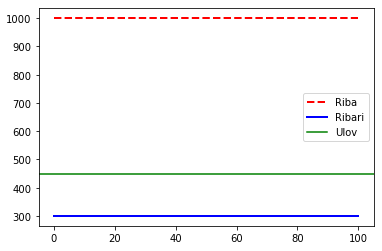
\includegraphics[width=10cm,height=4.5cm]{images/optimal1.png}
	\caption{Популација рибе, рибара и улов}
	\label{optimal}
\end{figure}

Помоћу добијене формуле за почетну популацију рибе од 1000, како би смо успоставили равнотежу потребно нам је 300 рибара који ће ловити 450 риба што можемо видети на слици \ref{optimal}, при чему је интензитет риболова 0.0015 а остали пареметри су остали исти као код других симулација. Како је и у примеру показано сада за било који број риба можемо одредити оптималан улов и број рибара тако да систем стално буде у стању равнотеже.

Треба имати у виду да је решење овог проблема локалног типа у односу на почетно задату популацију рибе са тежњом да популација рибе буде блиска жељеној вредности. У наредном поглављу ћемо видети да уколико се параметар интензитета риболова доста разликује од "равнотежног" интензитета за почетне популације рибе и рибара добијамо занимљиве резултате, и да горе описано решење не даје глобални оптимум у случају када дозвољавамо велике промене популације рибе и рибара у односу на почетне. Такоће треба тражити оптималне параметре унутар оптималног еквилибријума, за који се помоћу експерименталних резултата из наредног поглавља показало да се налази негде на средини интервала популације рибе.

\section{Количина улова у односу на интензитет риболова}
\label{sec:fishingintensity}
 Видели смо да у претходном поглављу да нам је један од најинтересантнијих параметра модела интензитет риболова. У овом делу ћемо помоћу експерименталних резултата продискутовати како промена интензитета риболова утиче на количину уловљене рибе, али и на популације рибе и рибара. 
 
\begin{figure}[h!]
	\centering
	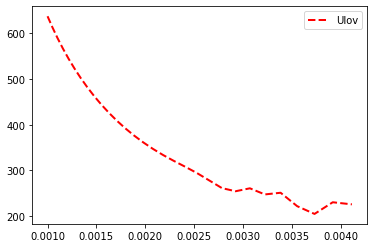
\includegraphics[width=10cm,height=4.5cm]{images/intensityIncrease.png}
	\caption{Количина уловљене рибе са порастом интензитета риболова}
	\label{intensityincrease}
\end{figure}
 
На слици \ref{intensityincrease} можемо видети како се мења просечна количина уловљене рибе на 100 година у односу на повећање интензитета риболова. За почетне параметре узето је стање еквилибријума са популацијом рибе од 1500, популацијом рибара од 425 и интензитетом риболова од 0.001, симулирано је повећање итензитета риболова док су сви остали параметри остали исти. Можемо приметити са графика очигледно опадање количине уловљене рибе како се интензитет повећава у односу на почетни параметар. Такоће видимо и благе скокове на графику који су последица упадања у нове тачке еквилибријума јер због велике промене интензитета почетни еквилибријум постаје нестабилан и велике осцилацији убацују модел у зону новог еквилибријума на основу тренутних популација рибе и рибара, али бољи такав пример ћемо продискутовати на графику са смањењем итензитета риболова. Без обзира на одскакања у неким деловима повећање интензитета риболова ће довести до истребљења популације рибе.

\begin{figure}[h!]
	\centering
	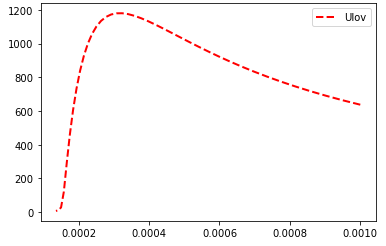
\includegraphics[width=10cm,height=4.5cm]{images/intensityDecrease.png}
	\caption{Количина уловљене рибе са смањењем интензитета риболова}
	\label{intensitydecrease}
\end{figure}

Утацај смањења интензитета риболова приказан је на слици \ref{intensitydecrease}, приметимо да график треба посматрати с десна на лево јер су интензитети приказани у растућем поретку. Са слике можемо видети да смањен итензитет риболова доводи до истребљења популације рибара а самим тим и улова. Занимљиво је да на почетку видимо раст уловљене рибе са смањењем интензитета риболова. До овога долази због нестабилности почетног еквилибријума и упадања у нове оптималније еквилибријуме који оквирно на средини интервала као што можемо видети на слици \ref{bettersolution}. 

\begin{figure}[h!]
	\centering
	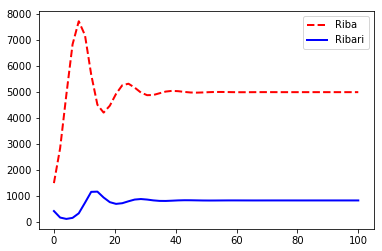
\includegraphics[width=10cm,height=4cm]{images/betterSolution.png}
	\caption{Упадање у нови еквилибријум}
	\label{bettersolution}
\end{figure}

Приметимо да на добијене резултате доста утиче одабир почетне популације рибе и рибара који је код нас био на почетку интервала, и да би одабиром популација са краја интервала добили обрнуте резултате тј. повећање интензитета би до неке вредности повећавало број уловљене рибе, а смањење интензитета би га смањило, али евентуално би и доста мале као и доста велике вредности интензитета довеле до нарушавања равнотеже и истребљења једне од врста.

\section{Закључак}
\label{sec:final}
Модификованим математичким моделом Лотка-Волтера смо описали популацију рибе и рибара, а затим смо продискутовали стања равнотеже модела. Закључили смо да је за жељену популацију рибе интензитет риболова и број рибара најбоље одредити на основу формуле еквилибријума. Посматрањем утицаја промене интензитета риболова на количину уловљене рибе видели смо да велики утицај игра одабрана почетна популација рибе, и да груби глобални оптимум налазимо негде на средини интервала, док локални оптимум проналазимо у еквилибријуму. У зависности од познатих и жељених параметара(почетна полулација рибе, популација рибара, интензитет риболова, или количина уловљене рибе) у стању смо да на основу њих одрадимо и остале параметре тако да систем буде уравнотожен. Препоручује се даље усавршавање овог проблема истраживање зарад проналаска ефикаснијих решења за одређивање оптимума али и усавршавање наведених. Такође треба имати на уму да наведени модел није идеалан и да постоји још модела и модификација који боље описују проблем грабљивац-плен. На крају можемо закључити да постоје много напредније и комплексније технике које овде нису наведе, а читалац се охрабрује да се упусти у ту авантуру и евентуално их унапреди и донесе неке нове закључке.

\nocite{mathmodeling}
\nocite{fishhavresting}
\nocite{fishanalysis}
\nocite{predatory}
\nocite{optimalhavrest}
\nocite{lotkavoltera}
\nocite{limitedgrowth}

\addcontentsline{toc}{section}{Литература}
\appendix
\bibliography{Fishing} 
\bibliographystyle{plain}
\newpage-
\end{document}
